\documentclass[conference]{IEEEtran}
\usepackage{cite}
\usepackage{amsmath,amssymb,amsfonts}
\usepackage{graphicx}
\usepackage{textcomp}
\usepackage{xcolor}
\usepackage{booktabs}
\usepackage{tabularx}
\usepackage{pifont}
\usepackage{hyperref}
\usepackage{enumitem}
\hypersetup{colorlinks=true, linkcolor=blue, citecolor=blue, urlcolor=blue}

% Author-facing marker. Search for \TODO before submission.
\newcommand{\TODO}[1]{\textcolor{red}{[\textbf{TODO:} #1]}}
% Figure helper: shows the image if the file exists, otherwise a labelled placeholder box.
\newcommand{\figfile}[3]{\IfFileExists{#1}{\includegraphics[width=#2]{#1}}{\fbox{\parbox{#2}{\centering\small\TODO{add \detokenize{#1}: #3}}}}}

\begin{document}

\title{\LARGE \bf Does the Court's Reasoning Give the Answer Away? An Ablation Audit of a Judgment Prediction Model on Indian Appeals}

\author{
\IEEEauthorblockN{Smruthi B S, Subashri V, Thanushree C B, Vidyashree M B, Dr. Mohammad Asif Raibag}
\IEEEauthorblockA{\textit{Department of Computer Science and Engineering (AI\,\&\,ML)} \\
\textit{PES University}, Bengaluru, India \\
\texttt{email@example.com}}
}

\maketitle

\begin{abstract}
Legal judgment prediction (LJP) models are usually judged by held-out accuracy, which cannot show whether a model reads the facts of a case or reads text that already states the outcome. We audit one trained model, a hierarchical InLegalBERT + BiGRU classifier for accepted-versus-rejected appeals, with inference-only tests. Each judgment is split into rhetorical roles with OpenNyAI, and the frozen model is fed the facts plus one role at a time, graduated mixtures of roles, and controlled edits of the text. On 1,308 PredEx test cases, facts alone give 49.4\% accuracy (AUC 0.62), and the model predicts ``rejected'' for 87\% of cases. Adding only the court's analysis sentences raises accuracy to 70.3\% (AUC 0.81), close to the full text (71.5\%, AUC 0.83). Statutes and section numbers add nothing. Controls show the effect is not length alone: at equal word counts only court reasoning moves predictions toward the true outcome, the last words of the analysis matter most, and when another case's analysis is placed after a case's own facts, the prediction follows that analysis's outcome (a shift of 0.31 in probability). Integrated Gradients attribution is dominated by position in the document, and expert rationales are 80\% analysis text, so explanation overlap with experts rewards this behaviour instead of exposing it. These results show that this model relies on post-decisional text, which does not exist when a prediction is needed. They do not show that facts carry no signal, nor that other models behave the same way; the model was also trained on Supreme Court criminal cases and tested on a mixed, mostly High Court set. We present the audit as a reusable procedure and list the controls we did not run.
\end{abstract}

\begin{IEEEkeywords}
Shortcut Learning, Legal Judgment Prediction, Outcome Leakage, Rhetorical Roles, Model Auditing, Integrated Gradients, InLegalBERT.
\end{IEEEkeywords}

\section{Introduction}
\label{sec:intro}
A judgment prediction system is only useful if it predicts before the judgment exists. Yet the text commonly used to train and test such systems is the judgment itself, which contains the court's reasoning and often its conclusion \cite{medvedeva2023mcbride}. A model can then score well by reading the reasoning rather than the case. This is an instance of shortcut learning \cite{geirhos2020shortcut}: a model solves a benchmark with a cue that is predictive in the data but is not what we want it to use. Neural networks also tend to favour the simplest predictive feature available \cite{shah2020pitfalls}, so an easy cue such as a sentence that states or implies the verdict is exactly what a trained model is likely to pick up.

Held-out accuracy cannot expose this. A shortcut-reliant model scores well on a test set drawn from the same distribution as its training data, because the cue is present in both. The problem only appears when the cue is removed or when the model is used where the cue does not exist \cite{steinmann2024navigating}. For judgment prediction, that is the real deployment setting: before a ruling, there is no reasoning section to read.

This concern is documented for legal prediction. Watson et al.\ \cite{watson2026shortcut} report that on UK Employment Tribunal data, strong headline accuracy is partly explained by outcome-revealing language in judicial text. We ask the same question for Indian appellate cases at a finer grain: which part of a judgment carries the signal, whether that is an effect of content or only of length and position, and whether common explanation methods would have caught it.

We study one model and make four contributions.
\begin{enumerate}[leftmargin=*]
    \item \textbf{An audit procedure.} We segment each judgment into rhetorical roles and run inference-only tests on a frozen model: a dose--response test, a one-role-at-a-time test, and a counterfactual test on section numbers (Section~\ref{sec:audit}, Fig.~\ref{fig:pipeline}). Nothing is retrained.
    \item \textbf{A case-study result.} For a hierarchical InLegalBERT model, the court's analysis sentences account for nearly all of its accuracy. Statutes, precedents, arguments, issues and rulings do not (Section~\ref{sec:results}).
    \item \textbf{Controls that separate content from length and position, and that test whether the model follows the outcome.} Six control experiments with exact word budgets, leave-one-role-out deletions, and transplanted analysis text (Section~\ref{sec:controls}).
    \item \textbf{A comparison with an explanation method.} Integrated Gradients and expert-rationale overlap on the same model, showing that they cannot detect this shortcut on their own (Section~\ref{sec:ig}).
\end{enumerate}
We also state which conclusions the evidence does not support, including that we have no facts-only trained model, only one checkpoint, and a test set whose domain differs from the training data (Section~\ref{sec:limits}).

\section{Background}
\label{sec:background}
\textbf{Shortcuts and spurious correlations.} Following Steinmann et al.\ \cite{steinmann2024navigating}, a correlation between an input feature and the label is \textit{spurious} when the feature is not one that should solve the task, and a \textit{shortcut} is a decision rule that uses it. They separate world-induced correlations, which exist in the real world, from sampling-induced ones, which arise from how a dataset was collected or filtered. Text in a published judgment that states the outcome is of the second kind for a prediction task: it is in the training data because the dataset was built from decided cases, and it is absent when a lawyer needs a prediction.

\textbf{Rhetorical roles and post-decisional text.} Legal judgments are long and have a typical structure. Rhetorical role labelling assigns each sentence a function such as facts, arguments, precedents, or the court's reasoning \cite{bhattacharya2019identification, nigam2025legalseg}. We use the OpenNyAI labeller \cite{kalamkar2022corpus}, which assigns one of 13 roles: preamble, facts (FAC), ruling by lower court (RLC), issue, arguments of petitioner and respondent, analysis, statute (STA), precedent relied and not relied, ratio, ruling by present court (RPC), and none. Roles let us separate content written \textit{before} the court reasons (facts, arguments) from content that reflects its reasoning or outcome. We call analysis, ratio and the present-court ruling \textit{post-decisional} text. This is legitimate legal reasoning, not noise; the problem is only that it is written after, and because of, the decision. We avoid the word ``spurious'' for these roles for that reason.

\textbf{Why input ablation.} Changing the input and watching the prediction is a direct, model-agnostic test of dependence, so it is our primary tool. Attribution methods are an obvious alternative. LIME \cite{ribeiro2016why} and SHAP \cite{lundberg2017unified} are approximate and costly on documents of thousands of tokens, attention is not reliable evidence of importance \cite{jain2019attention}, and probing shows what is encoded, not what is used \cite{belinkov2022probing}. Integrated Gradients (IG) \cite{sundararajan2017axiomatic} is a gradient-based method with a completeness property: attributions to the input words sum to the difference between the model's output on the input and on a baseline input. We use it as a comparison in Section~\ref{sec:ig} to ask whether a standard explanation method would have revealed what the behavioural tests found.

\section{Related Work}
\label{sec:related}
\textbf{Shortcut learning in NLP.} Shortcuts and annotation artifacts are well documented, for example hypothesis-only baselines for inference \cite{poliak2018hypothesis, gururangan2018annotation}, shallow syntactic heuristics \cite{mccoy2019right}, and cue words that explain BERT's accuracy on argument reasoning \cite{niven2019probing}. Geirhos et al.\ \cite{geirhos2020shortcut} give a general account, and Du et al.\ \cite{du2023shortcut} review it for language models. Diagnostics hold the task fixed while breaking the cue, as in contrast sets \cite{gardner2020contrast} and the shortcut suite of Yuan et al.\ \cite{yuan2024shortcut}. None of these contain legal text. Mitigation methods such as COMI \cite{zhao2024comi} and InterpoLL \cite{korakakis2025interpolated} assume a known shortcut; our audit addresses the earlier step of finding out whether one is present.

\textbf{Leakage in legal prediction.} Medvedeva et al.\ \cite{medvedeva2023rethinking} and Medvedeva and McBride \cite{medvedeva2023mcbride} argue that most LJP work trains on facts or text taken from published judgments, which are written after the decision. In a review of over 150 papers, they find that only about 7\% are doing what they set out to do, predicting court decisions \cite{medvedeva2023mcbride}. Watson et al.\ \cite{watson2026shortcut} study shortcut learning explicitly on UK Employment Tribunal claims and show that outcome-revealing language inflates performance, although much of the performance survived when it was masked in training. Chen et al.\ \cite{chen2023knowledge} find that a Legal-BERT model's important keywords concentrate on punctuation and function words, and Raj and Devi \cite{raj2023adversarially} show that synonym substitutions sharply reduce accuracy on ILDC. Our work differs in jurisdiction, in the use of role-level ablations and controls on a trained long-document model, and in that we evaluate a model rather than a feature set.

\textbf{Indian legal NLP.} ILDC \cite{malik2021ildc} introduced court judgment prediction with explanation for Indian Supreme Court cases, and IL-TUR \cite{joshi2024iltur} collects Indian legal benchmarks. InLegalBERT \cite{paul2023pre} is pre-trained on Indian legal text, following LEGAL-BERT \cite{chalkidis2020legalbert} for other jurisdictions. PredEx \cite{nigam2024predex} provides appellate cases with outcome labels and expert explanations. Later work narrows inputs to facts \cite{nigam2025tathyanyaya}, adds retrieved statutes and precedents \cite{patnaik2025nyayarag}, or evaluates LLMs in a more realistic setting \cite{nigam2024rethinking}. Fact-only inputs reduce leakage but are still extracted from judgments \cite{medvedeva2023mcbride}.

\textbf{Rhetorical roles in prediction.} Role labelling is a mature task on Indian judgments \cite{nigam2025legalseg}. Khatri et al.\ \cite{khatri2025structured} use roles at inference time as prompt structure for zero-shot LJP, and report in an ablation that removing the preamble hurt performance, which they attribute to reliance on metadata such as party names. We use roles differently: as a way of splitting the input to measure which part a trained model depends on.

\section{Model and Data}
\label{sec:model}
\textbf{Model.} Each judgment is split into 512-token chunks with stride 256 and at most 16 chunks (about 4.3k tokens). InLegalBERT encodes each chunk and the \texttt{[CLS]} vectors are passed to a 2-layer bidirectional GRU (hidden size 256, dropout 0.3). A linear layer outputs accepted or rejected (Fig.~\ref{fig:arch}). This hierarchical design follows the long-document approach used for ILDC \cite{malik2021ildc}. The last three BERT layers and the pooler are fine-tuned (24.6M of 112.2M parameters). We train on the criminal subset of ILDC/IL-TUR CJPE (7,094 training and 154 development cases). Development macro-F1 is 0.732, against 0.548 for a frozen-encoder baseline. \TODO{VERIFY F1 and parameter counts against the training notebook.}

\begin{figure}[t]
\centering
\figfile{figures/architecture.png}{0.95\columnwidth}{architecture diagram: judgment text, 512-token chunks, InLegalBERT, [CLS] vectors, BiGRU, linear layer, accepted/rejected}
\caption{The audited model. A judgment is chunked, each chunk is encoded by InLegalBERT, the \texttt{[CLS]} vectors are aggregated by a BiGRU, and a linear layer predicts accepted or rejected.}
\label{fig:arch}
\end{figure}

\textbf{Test data.} We evaluate on PredEx test cases. Overlap with ILDC training and development data was removed with a sliding-window matcher (300-character windows, step 150, on normalised text), which flagged 18 cases; 15 of the 18 flagged pairs have TF-IDF cosine similarity above 0.7 and three need manual review. This verification is weak: in a sample of 20 unflagged cases, 10 also scored above 0.7 against the flagged ILDC documents, so the threshold does not separate duplicates from topically similar judgments. The removal left 1,346 cases, and a stricter re-check is pending (Section~\ref{sec:limits}). The ablations use the 1,308 of these that contain at least one sentence tagged as facts. Of these, 738 (56.4\%) are accepted and 570 (43.6\%) are rejected, so a majority-class predictor scores 56.4\%.

\textbf{Domain mismatch.} The training data are ILDC criminal cases, which are Supreme Court judgments. The PredEx test set is a different distribution: according to the dataset's court field, 1,232 of the 1,346 cases (91.5\%) are High Court judgments and 114 are Supreme Court, and many case names indicate civil or commercial disputes. We did not filter the test set to criminal cases. Any result below therefore mixes shortcut reliance with distribution shift, and we cannot yet separate the two.

\section{Audit Procedure}
\label{sec:audit}
OpenNyAI tags every sentence with one of 13 roles. Every variant is built from ordered sentences, so text keeps its original document order, and all variants are scored on the same cases by the same frozen model (Fig.~\ref{fig:pipeline}).

\begin{figure}[t]
\centering
\figfile{figures/audit_pipeline.png}{0.95\columnwidth}{pipeline diagram: judgment, then OpenNyAI roles, then variants (facts only; facts plus one role; facts plus a growing share of the pool; section-number swap), then frozen model, then accuracy, shift and McNemar}
\caption{The audit pipeline. A judgment is split into roles, variants are built from ordered sentences, the frozen model scores each variant, and accuracy and prediction shift are compared with facts-only.}
\label{fig:pipeline}
\end{figure}

\subsection{Role ablations}
\textbf{Dose--response.} Facts plus a nested random subset (25, 50, 75 or 100\%) of a pool of outcome-adjacent roles: statutes, relied and not-relied precedents, lower-court ruling (RLC), present-court ruling (RPC) and analysis. One fixed shuffle per case keeps doses nested. Analysis sentences make up about three quarters of the pooled sentences across the test set (68,338 of 90,557 in the segmentation cache), so each dose is mostly analysis text, and dose is also confounded with added length. If the model used only facts, accuracy would stay flat as the dose grows.

\textbf{One role at a time.} Facts plus exactly one role group: analysis, arguments, RLC, precedents, ratio, statutes, issues, or RPC. Arguments are a pre-outcome control: they are written before the court reasons, so a model that reads the case should not gain from them much more than it does from other pre-outcome text.

\textbf{Counterfactual.} Statute section numbers inside the facts are replaced by one fixed number (144), and, separately, inside the statute sentences as well. We also mask a wider set of legal references (section references, outcome words, citations, act names and court names) in the facts. If the model relied on specific section numbers as cues, predictions should move.

\textbf{Baselines.} The segmented full text and the raw judgment text.

\subsection{Control experiments}
\label{sec:controls}
The role ablations leave open three objections: analysis is simply the longest role, the facts-only input is unlike anything the model was trained on, and a changed prediction may not mean the model follows the content. Six controls, defined before they were run, address these. All use the same model and cases.
\begin{itemize}[leftmargin=*]
    \item \textbf{A. No facts.} Roles are fed without the facts. If analysis alone approaches the raw-text accuracy, the facts are not needed.
    \item \textbf{B. Leave one role out.} A role is deleted from near-full documents and compared with deleting the same number of random words. This tests whether the role is necessary, in inputs closer to the training distribution.
    \item \textbf{C. Exact word budgets.} The first 60 or 150 words of a role, or the last 60 or 150, are added to the facts at a fixed position. Controls add repeated facts or facts from another case, which add length but no new information about this case. Analysis start and end are compared directly.
    \item \textbf{D. Transplant.} The facts stay fixed and another case's analysis (or statute, precedent, arguments, RLC) text is added. We compare the model's P(accepted) when the donor case was accepted with when it was rejected. A model that follows the outcome written in the text will show a positive difference.
    \item \textbf{E. Noise floor.} Section-number swaps are compared with a harmless edit, dropping one random sentence.
    \item \textbf{F. Dose without analysis.} The dose--response curve is rerun with analysis removed from the pool.
\end{itemize}

\subsection{Explanation-based check}
\label{sec:igproc}
For all 1,346 cases we compute Integrated Gradients \cite{sundararajan2017axiomatic} on the decision margin (the predicted logit minus the other logit), with a padding-token baseline, 32 steps, and a recomputation at 128 steps when the completeness error exceeds 5\% of the output gap. Word-level attributions are summed within each rhetorical role and compared with the role's share of words. Because attribution turns out to depend strongly on where text sits in the document, we also report a \textit{position-adjusted} ratio: each word's attribution divided by what pre-decision text (facts, arguments, statutes, precedents, lower-court ruling) receives at the same relative position across all cases, so a value of 1 means ``what its position predicts''. We then compare the model's top-attributed words with the PredEx expert rationale by intersection over union (IoU), against random words and against random words with the same role mix as the model's top words.

\subsection{Measures}
We report accuracy, AUC, and the \textit{shift rate}, the fraction of cases whose prediction differs from the facts-only prediction. Some roles are absent from many cases (the RPC variant's text equals the facts-only text in 75\% of cases, statutes in 59\%), which dilutes an all-case shift rate. We therefore also report the shift rate over cases where the variant text differs from its baseline, with the number of such cases and Wilson 95\% intervals. Accuracy differences between variants on the same cases use the exact two-sided McNemar test; contrasts in the control experiments use paired bootstrap intervals over cases. The McNemar $p$-values in Tables~\ref{tab:dose} and~\ref{tab:roles} are uncorrected, and a non-significant result is not evidence of equivalence. The main effects are far below any usual correction threshold; borderline ones (for example arguments, $p=0.036$) should not be read as significant.

\section{Results}
\label{sec:results}

\begin{figure*}[t]
\centering
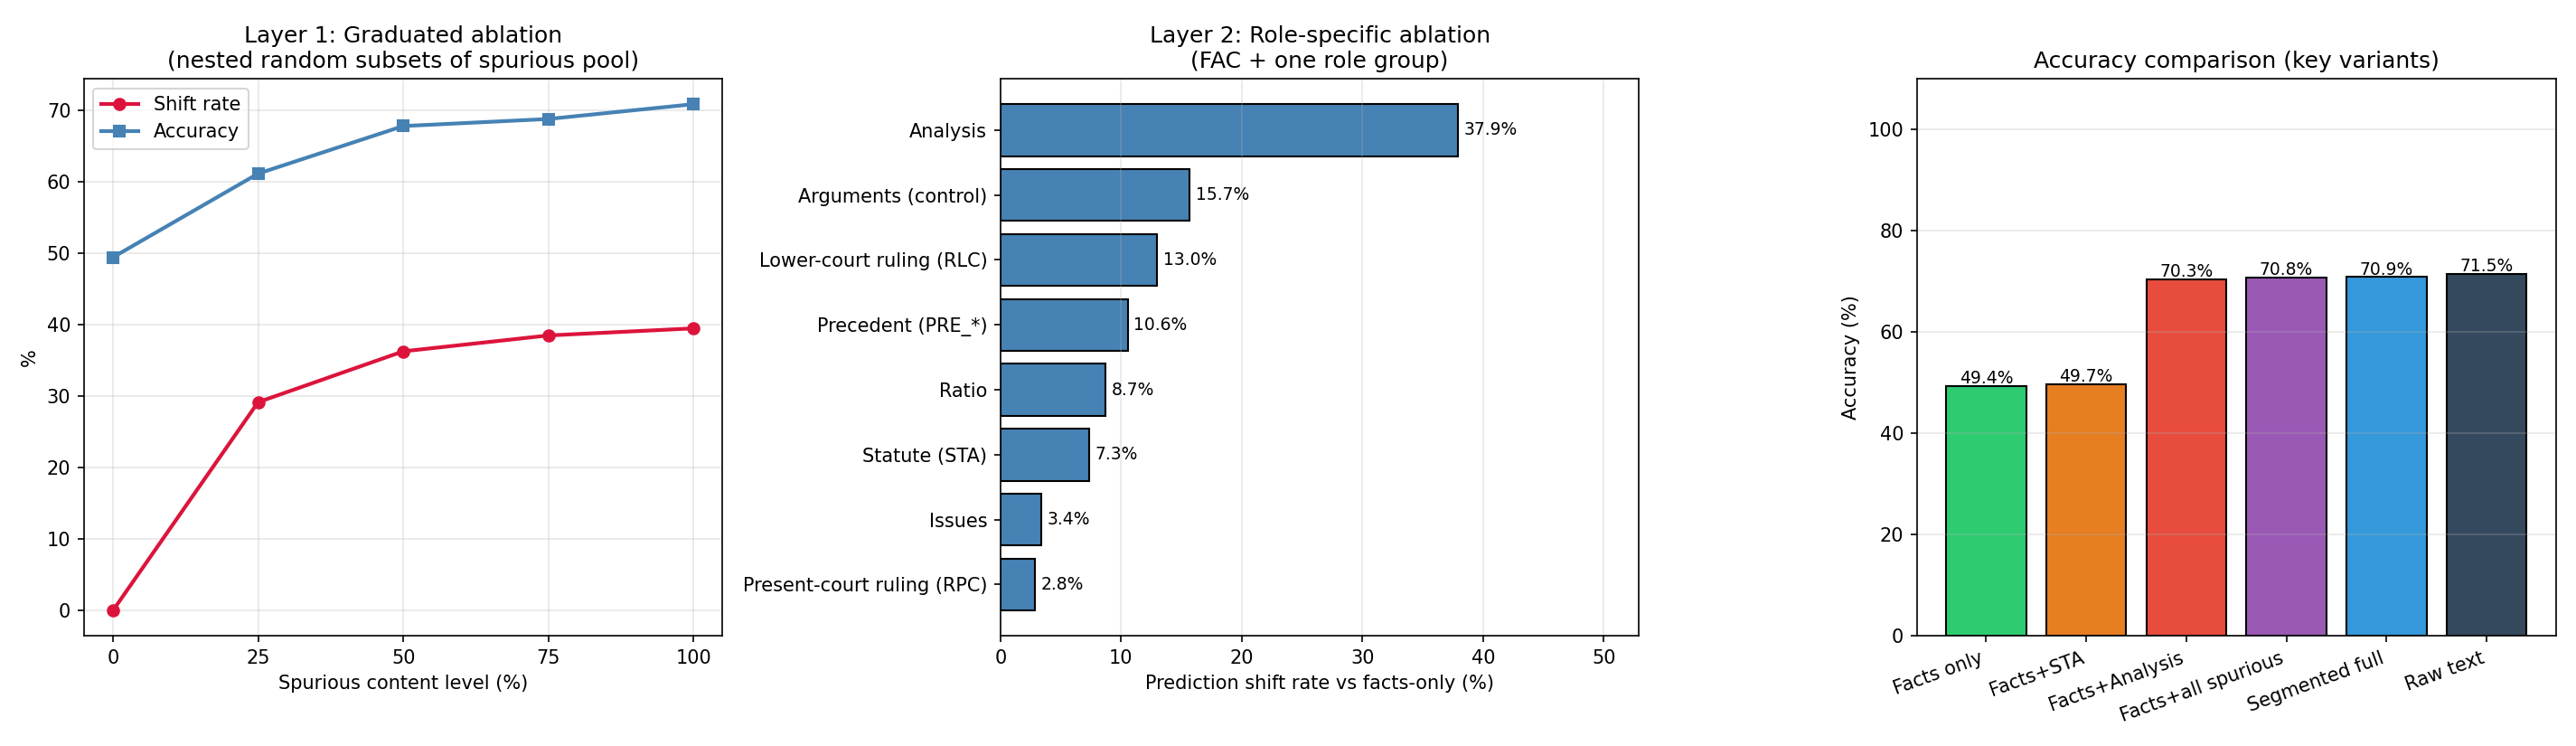
\includegraphics[width=\textwidth]{figures/combined_ablation_v2.png}
\caption{Ablation results. Left: dose--response. Middle: shift rate over all cases by role. Right: accuracy of key variants.}
\label{fig:combined}
\end{figure*}

\subsection{Role ablations}
\textbf{Facts alone are not enough for this model.} With facts only, accuracy is 49.4\%, below the 56.4\% majority baseline. The model predicts ``rejected'' for 1,136 of 1,308 cases (86.9\%); recall is 91.6\% on rejected cases (522/570) and 16.8\% on accepted cases (124/738). The model has collapsed to a near-constant prediction on this input, so accuracy near 50\% should not be read as chance-level reasoning about the facts. A rank-based view is less harsh: facts-only AUC is 0.62, and moving the decision threshold to the base rate gives 60.1\% accuracy. Facts carry a weak signal that the default threshold hides. We therefore compare variants by AUC as well as accuracy.

\textbf{Accuracy rises with outcome-adjacent text.} Accuracy climbs from 49.4\% to 61.1\%, 67.7\%, 68.7\% and 70.8\% across the four doses (Table~\ref{tab:dose}, Fig.~\ref{fig:combined}), and AUC from 0.62 to 0.81; every step over facts-only is significant ($p<10^{-14}$). The curve is steepest at the first dose. Because the pool is mostly analysis text, this is consistent with a single dominant role rather than many weak ones, but the dose experiment alone cannot show that.

\begin{table}[t]
\caption{Dose--response. Shift is over all 1,308 cases; $p$ compares accuracy with facts-only.}
\label{tab:dose}
\centering
\small
\begin{tabular}{lrrr}
\toprule
\textbf{Variant} & \textbf{Acc.\ (\%)} & \textbf{Shift (\%)} & \textbf{McNemar $p$} \\
\midrule
Facts only & 49.4 & -- & -- \\
+25\% & 61.1 & 29.1 & $3\times10^{-15}$ \\
+50\% & 67.7 & 36.2 & $3\times10^{-29}$ \\
+75\% & 68.7 & 38.5 & $1\times10^{-30}$ \\
+100\% & 70.8 & 39.4 & $2\times10^{-36}$ \\
\bottomrule
\end{tabular}
\end{table}

\textbf{Analysis carries the signal.} Adding only the analysis sentences gives 70.3\% accuracy and AUC 0.81 (Table~\ref{tab:roles}). We find no significant difference from the full pool (70.8\%, $p=0.72$) or from the raw text (71.5\%, $p=0.38$), and it is far above the arguments control ($p\approx10^{-29}$). Among the 496 predictions it flips, 385 (78\%) move toward the true label. The flips are mostly from rejected to accepted, so about 56\%, the accepted-class share, would be expected if flips were unrelated to the label. Recall on accepted cases rises from 16.8\% to 61.5\%, while recall on rejected cases falls from 91.6\% to 81.8\%.

\begin{table*}[t]
\caption{One role at a time. $n$ changed is the number of cases where the added role changes the text; shift is computed over those cases. Accuracy is over all 1,308 cases. The $p$-values are uncorrected.}
\label{tab:roles}
\centering
\small
\begin{tabular}{lrrrrr}
\toprule
\textbf{Role added to facts} & \textbf{$n$ changed} & \textbf{Acc.\ (\%)} & \textbf{Shift, changed (\%)} & \textbf{95\% CI} & \textbf{McNemar $p$} \\
\midrule
Analysis & 1291 & 70.3 & 38.4 & 35.8--41.1 & $2\times10^{-36}$ \\
Arguments (control) & 961 & 51.8 & 21.3 & 18.9--24.0 & 0.036 \\
Statutes & 530 & 49.7 & 18.1 & 15.1--21.6 & 0.76 \\
Precedents & 767 & 52.4 & 18.0 & 15.4--20.9 & $8\times10^{-4}$ \\
Ratio & 644 & 53.2 & 17.7 & 14.9--20.8 & $3\times10^{-6}$ \\
Lower-court ruling (RLC) & 1074 & 51.1 & 15.8 & 13.8--18.1 & 0.11 \\
Issues & 305 & 50.3 & 14.4 & 10.9--18.8 & 0.096 \\
Present-court ruling (RPC) & 333 & 49.8 & 11.1 & 8.2--14.9 & 0.51 \\
\bottomrule
\end{tabular}
\end{table*}

\textbf{No other role comes close.} Apart from analysis, every role shifts predictions in 11--21\% of the cases where it is present, with overlapping intervals, so we do not rank them against each other. Ratio and precedents give small but significant accuracy gains (53.2\% and 52.4\%); the others do not differ significantly from facts-only at the 0.01 level. Statute text adds +0.3 points of accuracy (95\% CI $-1.2$ to $+1.8$) and no AUC.

\textbf{Section numbers: no sign of reliance in this test.} Replacing section numbers in the facts changes 4.1\% of predictions (95\% CI 3.0--5.6, $n=884$ cases containing a section number) and leaves accuracy unchanged (49.4\%, $p=1.0$). Applying the swap inside the statute sentences as well changes 5.3\% ($n=956$ changed cases). Masking a wider set of legal references in the facts shifts 9.3\% ($n=1{,}123$) with no accuracy gain. These tests use inputs on which the model is already near-constant, so on their own they have little power to show reliance; Control E below gives a noise floor, and a swap applied to inputs where the model performs well (for example facts plus analysis) has not been run.

\textbf{Baselines.} The segmented full text scores 70.9\% and the raw judgment 71.5\%. Analysis alone therefore recovers essentially all of the full-text accuracy.

\subsection{Control experiments}
Table~\ref{tab:controls} summarises the six controls; each supports the same reading.

\begin{table*}[t]
\caption{Control experiments (1,308 cases, paired bootstrap 95\% intervals in brackets). ``Toward truth'' is the mean change in the model's probability of the correct outcome.}
\label{tab:controls}
\centering
\small
\begin{tabularx}{\textwidth}{lX}
\toprule
\textbf{Control} & \textbf{Result} \\
\midrule
A. No facts & Analysis alone: 70.0\% accuracy, AUC 0.805 (raw text 71.5\%, 0.828). All roles without facts: 72.1\%, AUC 0.826. All non-analysis roles without facts: 52.8\%, AUC 0.604. \\
B. Leave one out & Removing analysis lowers accuracy by 11.3 points [$-14.1$, $-8.6$] against 3.9 for deleting the same number of random words; excess drop in the model's output 0.043 [0.030, 0.056]. Removing statute text is about the same as random deletion (excess $-0.010$ [$-0.022$, 0.002]) and raises accuracy by 3.6 points [0.8, 6.8] on the 530 cases that have statute text. \\
C. Word budgets (150 words) & Toward truth: last 150 words of analysis +7.1 points [6.0, 8.1]; first 150 words +2.5; whole analysis role +4.3; precedent +1.6; arguments +1.4; statute +1.1 [$-0.0$, 2.2]; repeated facts $-0.3$; facts from another case $-0.6$. At 60 words ratio is highest (+4.0), with the last 60 words of analysis (+3.3) above every other role. \\
D. Transplant & P(accepted$\mid$donor accepted) $-$ P(accepted$\mid$donor rejected): analysis \textbf{0.310} [0.291, 0.331]; precedent 0.076, arguments 0.080, RLC 0.035, statute 0.032 [0.025, 0.039]. The prediction follows the donor's outcome in 46.9\% of cases and goes against it in 6.0\% for analysis. \\
E. Noise floor & Section-number swaps flip 3.8--5.0\% of changed cases in the facts; dropping one random facts sentence flips 8.7\%. On raw text, swaps flip 5.8--6.1\% against 8.4\% for one dropped sentence. \\
F. Dose without analysis & Accuracy 49.4 $\rightarrow$ 52.6 $\rightarrow$ 52.4 $\rightarrow$ 54.2 $\rightarrow$ 55.5\% (AUC 0.62 $\rightarrow$ 0.66), against 70.8\% (0.81) with analysis in the pool. \\
\bottomrule
\end{tabularx}
\end{table*}

\textbf{Content, not only length.} Control C adds the same number of words from each source. At 150 words, the last of the analysis moves the prediction toward the truth by 7.1 points, while repeated facts and another case's facts, which add length but nothing relevant, move it by about zero. The end of the analysis also carries about three times the effect of its start (7.1 against 2.5), and a bag-of-words classifier with no neural encoder shows the same pattern (AUC 0.675 on the last 150 words of analysis against 0.603 on the first 150). The end of the analysis is the text just before the decision that the dataset removed.

\textbf{Necessary and sufficient, in different inputs.} Analysis alone nearly matches the raw text (Control A), and deleting it from near-full documents costs three times more than deleting random words of the same length (Control B). Statutes behave like noise in both tests.

\textbf{The model follows the outcome in the text.} In the transplant test (Fig.~\ref{fig:transplant}) the facts never change, only the donor's outcome does, yet P(accepted) moves by 0.31. The same test for statute text gives 0.03, about a tenth as much (small, with a confidence interval that excludes zero, so we do not call it zero).

\begin{figure}[t]
\centering
\figfile{figures/fig_controls_transplant.png}{0.95\columnwidth}{Control D: transplant effect by role}
\caption{Transplant control. The facts are fixed and another case's text is added. The bar is the difference in P(accepted) between donors that were accepted and donors that were rejected, with 95\% intervals.}
\label{fig:transplant}
\end{figure}

\subsection{Explanation-based check}
\label{sec:ig}
\textbf{Attribution favours post-decisional text, but position explains much of it.} Analysis, ratio and the present-court ruling hold 43\% of the words the model sees and 51\% of the attribution, while facts and statutes receive less than their share (Fig.~\ref{fig:ig}). This matches the behavioural result in direction. However, attribution is strongly U-shaped over the document: pre-decision text gets about 3.5 times the average attribution in the last 5\% of the visible document and about half the average in the middle. A plausible cause is the architecture, since the BiGRU's output is built from its final states, which sit at the last chunk (forward direction) and the first chunk (backward direction). Analysis is the long section that runs to the end of most judgments, so much of its excess is position. After the position adjustment (Table~\ref{tab:ig}), the analysis section as a whole is no longer favoured (0.96), but the short outcome-stating parts still are (ratio 1.49, present-court ruling 1.61), and statutes stay below (0.76). Arguments by the petitioner are also above 1 (1.48), which a leakage account does not predict: IG favours argumentative text in general.

\begin{figure}[t]
\centering
\figfile{figures/fig_role_attribution.png}{0.95\columnwidth}{IG attribution share vs word share by role}
\caption{Share of words and share of Integrated Gradients attribution by rhetorical role (mean over cases containing the role).}
\label{fig:ig}
\end{figure}

\begin{table}[t]
\caption{Integrated Gradients by role. Excess is attribution share minus word share (percentage points). Position-adjusted 1 means ``what its position predicts''. 95\% intervals in brackets.}
\label{tab:ig}
\centering
\small
\setlength{\tabcolsep}{3pt}
\begin{tabular}{lrrrr}
\toprule
\textbf{Role} & \textbf{Cases} & \textbf{Words} & \textbf{Excess} & \textbf{Pos.-adj.} \\
\midrule
Analysis & 1,310 & 41.7\% & +4.6 & 0.96 [0.95, 0.98] \\
Ratio & 416 & 3.6\% & +8.9 & 1.49 [1.40, 1.58] \\
Present-court ruling & 221 & 3.7\% & +5.5 & 1.61 [1.45, 1.77] \\
Facts & 1,306 & 28.9\% & $-6.2$ & 0.99 [0.98, 1.01] \\
Statute & 504 & 13.3\% & $-5.4$ & 0.76 [0.74, 0.79] \\
Arguments (petitioner) & 817 & 9.9\% & $-0.8$ & 1.48 [1.42, 1.53] \\
\bottomrule
\end{tabular}
\end{table}

\textbf{Within the analysis, start and end cannot be separated by IG.} The last 60 words of the analysis get about three times the average attribution and the first 60 about 0.7 times, but after position adjustment both are close to 1 (1.04 and 1.14). With full judgments, ``end of the analysis'' cannot be told apart from ``end of the document'', and in about a third of the cases that are long enough the end of the analysis lies outside the model's window. The controls above, which place the first and last analysis words at the same position, remain the evidence on this point.

\textbf{Expert agreement rewards the leakage.} The PredEx expert rationale is itself mostly post-decisional: of the visible expert-marked words, 79.6\% are analysis, 14.0\% ratio and 10.7\% present-court ruling, and only 2.0\% are facts (means over cases containing each role, so shares do not add to 100\%). The model's top attributed words reach an IoU of 0.267 [0.259, 0.274] with the expert rationale, against 0.166 for random words, but 0.216 for random words with the same role mix as the model's top words. About half of the model's advantage over random words therefore comes from both preferring the same roles; within roles the model still matches expert words slightly better than chance (+0.051 [0.047, 0.055]). On PredEx, high agreement with the expert rationale is what a model that reads the outcome from the court's reasoning would show. The measure rewards the leakage and cannot detect it.

\textbf{Per-case attribution barely tracks the behavioural result.} Across 1,272 cases, the Spearman correlation between a case's attribution excess on the analysis and the Stage-2 measures is $-0.03$ [$-0.08$, 0.03] for the probability gained by adding the analysis to the facts, $-0.06$ [$-0.11$, 0.00] for following a transplanted analysis, and $+0.10$ [0.04, 0.15] for the loss from deleting the analysis (leave-one-out, the control done on near-full documents like IG). Only the last is distinguishable from zero, and it is weak. IG's per-case attribution to the analysis is not a usable per-case detector of the reliance that the behavioural tests measure.

\textbf{Soundness checks.} Masking the 10\% of words IG ranks highest moves the decision margin 0.86 more than masking the lowest-ranked 10\% (95\% CI 0.79--0.93), and the gap is positive in 73\% of cases. The IG completeness error has a median of 2.3\% of the output gap; 83\% of cases are within 5\% and 4.5\% are above 10\%. Repeating the analysis on only the 1,121 cases within 5\% changes no conclusion. About a third of judgments (32.8\%) exceed the model's 16-chunk window, and all measures use only the text the model reads.

\section{Discussion}
\label{sec:discussion}
\textbf{What this says about the model.} On facts alone the model predicts one class for almost every case, and it recovers almost all of its full-text accuracy from the court's analysis. Analysis sentences are written after the court has decided, so a model that depends on them could not predict an appeal before it is decided. The controls move this from a description to something closer to a mechanism: the effect survives matching for length (C), is necessary in near-full documents (B), and the prediction follows the outcome of a transplanted analysis (D). We still call it post-decisional leakage as a description of model behaviour, and note it does not tell us which sentence inside the analysis the model uses. The pattern is the sampling-induced kind described in Section~\ref{sec:background}: the cue is in the data because the data are decided judgments.

\textbf{Distribution shift is an alternative reading of the facts-only result.} The model was trained on Supreme Court criminal cases and tested mostly on High Court cases, many of them civil or commercial. A model that falls back on one class for unfamiliar short inputs would also give the facts-only result we see. We therefore treat the collapse as a fact about this model on this test set, not as evidence about the information in case facts, and rely on AUC (0.62) for the weak signal facts do carry. The transplant and word-budget controls compare variants of the same input and are less exposed to this issue.

\textbf{Explanations are not an audit.} The IG results illustrate a practical point for legal AI. A system that showed attribution maps, or scored itself by overlap with expert rationales, would look reasonable here: the model attends to the court's reasoning, as the experts do. Yet that is exactly the shortcut. Position dominates the attributions, expert rationales are themselves post-decisional, and per-case attribution does not track reliance. Explanation-based audits of judgment prediction should control for position and for the composition of the rationale, and be paired with behavioural tests that change the input.

\textbf{Relation to earlier findings.} Watson et al.\ \cite{watson2026shortcut} find that models exploit leakage when it is available yet retain some signal when it is removed. Our facts-only result looks starker, but it is not comparable: their models were retrained with the cues masked, while ours was trained with them present and is then shown input without them. Medvedeva and McBride \cite{medvedeva2023mcbride} argue that benchmarks built on judgment text say little about prediction of future decisions; our results show one way that failure can look inside a single trained model. The role-level view also connects to Khatri et al.\ \cite{khatri2025structured}, who found that role structure changes LJP behaviour in a different setting (zero-shot LLMs), although we do not claim the two findings are the same phenomenon.

\textbf{Present-court ruling.} The model barely reacts to the tagged ruling sentences (11.1\% shift, no accuracy gain), yet reacts strongly to the analysis, while IG gives the same sentences 1.6 times what their position predicts. Ruling text is absent from most cases as tagged, and some outcome statements may sit inside analysis, so we do not read this as the model ignoring a stated verdict.

\textbf{Using the audit.} The procedure needs only a trained model, a test set and a role tagger. Its outputs are accuracy, AUC and shift per role with intervals and paired tests, a transplant difference, and optionally an attribution profile, all of which can be reported next to held-out accuracy and run before a model is trusted. We do not propose a deployment threshold and have not calibrated what shift level matters in practice.

\textbf{Implications for building LJP models.} A model should be evaluated on inputs available at prediction time, and pre-decision documents such as petitions and lower-court records are the sound choice \cite{medvedeva2023mcbride}. Where only judgments exist, the audit gives a way to measure how much of a model's accuracy comes from post-decisional roles, and training on facts only is the obvious next comparison.

\section{Limitations}
\label{sec:limits}
These are the main reasons the results should be read narrowly.
\begin{itemize}[leftmargin=*]
    \item \textbf{No facts-only model.} The model was trained on full text, so the facts-only variant is an input it was not built for. Its 49.4\% accuracy may reflect that mismatch rather than an absence of signal in the facts. A model trained on facts alone is needed to estimate what facts can predict.
    \item \textbf{Train--test domain mismatch.} Training is on Supreme Court criminal cases; the test set is 91.5\% High Court by the dataset's court field, with many non-criminal cases, and we did not filter it. Shortcut reliance and distribution shift are not separated.
    \item \textbf{One checkpoint.} We cannot say whether other seeds, architectures or encoders behave the same. The procedure is model-agnostic by design, but is shown on one model. The IG results are likewise for one attribution method and one baseline.
    \item \textbf{Content and position are only partly separated.} The word-budget controls match length and place text at a fixed position, which answers the main length objection. We did not test whether disposition sentences inside the analysis account for its effect, and we did not move the whole analysis before the facts. A sequential aggregator that weights later chunks remains a possible contributor, and IG shows strong position effects.
    \item \textbf{Role labels are unvalidated.} OpenNyAI's reported weighted F1 is about 0.78, and its tags were not checked by hand on this data. Verdict-like sentences may be tagged as analysis, which would make that variant a stronger leak than its label implies, and statute discussion may be tagged as analysis.
    \item \textbf{Overlap with training data.} Our ILDC--PredEx overlap removal was not fully validated. The TF-IDF check cannot separate duplicates from topically similar judgments, three of the 18 flagged pairs need manual review, and the fixed-offset window matcher may miss aligned copies. Some overlap may remain, which would inflate absolute accuracy.
    \item \textbf{Counterfactual power.} The section-number tests use inputs on which the model is near-constant, and section 144 is a real CrPC provision, so it is not a perfectly neutral replacement.
    \item \textbf{Truncation.} The model reads at most 16 chunks; about a third of judgments are longer, which may remove end-of-judgment text from the full-text variants and the end of the analysis in some cases.
    \item \textbf{Ablation changes the input.} Any removal shifts the input distribution, so some shift occurs regardless of content. The arguments control and the noise-floor control only partly bound this.
    \item \textbf{Scale and statistics.} One dataset, 1,308 cases. McNemar $p$-values in the main tables are uncorrected; differences among non-analysis roles are not statistically supported.
\end{itemize}

\section{Future Work}
\label{sec:future}
Five experiments would turn this case study into a stronger result. First, train a facts-only model and compare it with the full-text model on the same cases. Second, repeat the audit on a criminal-only subset of the test set to separate shortcut reliance from domain shift. Third, run the audit on several seeds and on other encoders, and repeat the explanation check with other baselines and methods. Fourth, remove disposition sentences from the analysis, move the analysis before the facts, and apply the section-number swap to facts plus analysis, to separate content from position and explicit verdict text. Fifth, validate OpenNyAI labels on a hand-checked sample and re-run the overlap check with word-level shingles against all ILDC training and development documents.

\section{Conclusion}
\label{sec:conclusion}
For one hierarchical InLegalBERT model on a mixed PredEx test set, accuracy comes almost entirely from the court's analysis sentences, which are written after the decision. The effect is not explained by length: at equal word counts only court reasoning moves predictions toward the truth, and a transplanted analysis moves the prediction toward its own outcome. Facts-only input collapses to a single predicted class, though facts carry a weak signal (AUC 0.62), and section numbers are not the cause. Integrated Gradients and expert-rationale overlap would not have flagged the problem, because attribution is dominated by position and the expert rationales are themselves post-decisional. The audit uses no retraining and reports paired tests and intervals. The open questions are whether facts carry signal when a model is trained on them, whether the facts-only collapse is partly distribution shift, and whether the effect holds across models.

\section*{Acknowledgment}
We thank our guide, Dr.\ Mohammad Asif Raibag. \TODO{add funding and compute acknowledgments.}

\begin{thebibliography}{99}
\bibitem{geirhos2020shortcut} R. Geirhos \textit{et al.}, ``Shortcut learning in deep neural networks,'' \textit{Nature Machine Intelligence}, vol. 2, no. 11, pp. 665--673, 2020.
\bibitem{du2023shortcut} M. Du \textit{et al.}, ``Shortcut learning of large language models in natural language understanding,'' \textit{Communications of the ACM}, vol. 67, no. 1, pp. 110--120, 2023.
\bibitem{dogra2024shortcut} V. Dogra, S. Verma, Kavita, M. Wo\'{z}niak, J. Shafi, and M. F. Ijaz, ``Shortcut learning explanations for deep natural language processing: A survey on dataset biases,'' \textit{IEEE Access}, vol. 12, pp. 26183--26195, 2024. \TODO{verify page range.}
\bibitem{steinmann2024navigating} D. Steinmann, F. Divo, M. Kraus, A. W\"{u}st, L. Struppek, F. Friedrich, and K. Kersting, ``Navigating shortcuts, spurious correlations, and confounders: From origins via detection to mitigation,'' \textit{arXiv preprint arXiv:2412.05152}, 2024.
\bibitem{gururangan2018annotation} S. Gururangan \textit{et al.}, ``Annotation artifacts in natural language inference data,'' in \textit{Proc. NAACL-HLT}, pp. 107--112, 2018.
\bibitem{niven2019probing} T. Niven and H.-Y. Kao, ``Probing neural network comprehension of natural language arguments,'' in \textit{Proc. ACL}, pp. 4658--4664, 2019.
\bibitem{mccoy2019right} R. T. McCoy, E. Pavlick, and T. Linzen, ``Right for the wrong reasons: Diagnosing syntactic heuristics in natural language inference,'' in \textit{Proc. ACL}, pp. 3428--3448, 2019.
\bibitem{yuan2024shortcut} Y. Yuan, L. Zhao, K. Zhang, G. Zheng, and Q. Liu, ``Do LLMs overcome shortcut learning? An evaluation of shortcut challenges in large language models,'' in \textit{Proc. EMNLP}, pp. 12188--12200, 2024.
\bibitem{sun2024exploring} Z. Sun, Y. Xiao, J. Li, Y. Ji, W. Chen, and M. Zhang, ``Exploring and mitigating shortcut learning for generative large language models,'' in \textit{Proc. LREC-COLING}, pp. 6883--6893, 2024.
\bibitem{baker2023explainable} S. Baker and W. Xiang, ``Explainable AI is responsible AI: How explainability creates trustworthy and socially responsible artificial intelligence,'' \textit{arXiv preprint arXiv:2312.01555}, 2023. \TODO{confirm venue; the draft listed IEEE Access.}
\bibitem{medvedeva2023mcbride} M. Medvedeva and P. McBride, ``Legal judgment prediction: If you are going to do it, do it right,'' in \textit{Proc. Natural Legal Language Processing Workshop 2023}, Singapore, pp. 73--84, 2023.
\bibitem{medvedeva2023rethinking} M. Medvedeva, M. Wieling, and M. Vols, ``Rethinking the field of automatic prediction of court decisions,'' \textit{Artificial Intelligence and Law}, vol. 31, no. 1, pp. 195--212, 2023.
\bibitem{cepej2018charter} European Commission for the Efficiency of Justice (CEPEJ), ``European ethical charter on the use of artificial intelligence in judicial systems and their environment,'' Council of Europe, Strasbourg, 2018.
\bibitem{patnaik2025nyayarag} S. K. Nigam, B. D. Patnaik, S. Mishra, A. V. Thomas, N. Shallum, K. Ghosh, and A. Bhattacharya, ``NyayaRAG: Realistic legal judgment prediction with RAG under the Indian common law system,'' \textit{arXiv preprint arXiv:2508.00709}, 2025.
\bibitem{gardner2020contrast} M. Gardner \textit{et al.}, ``Evaluating models' local decision boundaries via contrast sets,'' in \textit{Findings of EMNLP}, pp. 1307--1323, 2020.
\bibitem{warstadt2020blimp} A. Warstadt \textit{et al.}, ``BLiMP: The benchmark of linguistic minimal pairs for English,'' \textit{TACL}, vol. 8, pp. 377--392, 2020.
\bibitem{ko2020look} M. Ko, J. Lee, H. Kim, G. Kim, and J. Kang, ``Look at the first sentence: Position bias in question answering,'' in \textit{Proc. EMNLP}, pp. 1109--1121, 2020.
\bibitem{qi2021mind} F. Qi, Y. Chen, X. Zhang, M. Li, Z. Liu, and M. Sun, ``Mind the style of text! Adversarial and backdoor attacks based on text style transfer,'' in \textit{Proc. EMNLP}, pp. 4569--4580, 2021.
\bibitem{wei2022chain} J. Wei \textit{et al.}, ``Chain-of-thought prompting elicits reasoning in large language models,'' in \textit{Proc. NeurIPS}, vol. 35, pp. 24824--24837, 2022.
\bibitem{xiong2023can} M. Xiong \textit{et al.}, ``Can LLMs express their uncertainty? An empirical evaluation of confidence elicitation in LLMs,'' in \textit{Proc. ICLR}, 2024.
\bibitem{ribeiro2016why} M. T. Ribeiro, S. Singh, and C. Guestrin, ```Why should I trust you?': Explaining the predictions of any classifier,'' in \textit{Proc. ACM SIGKDD}, pp. 1135--1144, 2016.
\bibitem{garreau2020explaining} D. Garreau and U. von Luxburg, ``Explaining the explainer: A first theoretical analysis of LIME,'' in \textit{Proc. AISTATS}, PMLR vol. 108, 2020.
\bibitem{lundberg2017unified} S. M. Lundberg and S.-I. Lee, ``A unified approach to interpreting model predictions,'' in \textit{Proc. NIPS}, pp. 4765--4774, 2017.
\bibitem{selvaraju2017grad} R. R. Selvaraju \textit{et al.}, ``Grad-CAM: Visual explanations from deep networks via gradient-based localization,'' in \textit{Proc. IEEE ICCV}, pp. 618--626, 2017.
\bibitem{jain2019attention} S. Jain and B. C. Wallace, ``Attention is not explanation,'' in \textit{Proc. NAACL-HLT}, pp. 3543--3556, 2019.
\bibitem{tenney2019probing} I. Tenney \textit{et al.}, ``What do you learn from context? Probing for sentence structure in contextualized word representations,'' in \textit{Proc. ICLR}, 2019.
\bibitem{belinkov2022probing} Y. Belinkov, ``Probing classifiers: Promises, shortcomings, and advances,'' \textit{Computational Linguistics}, vol. 48, no. 1, pp. 207--219, 2022.
\bibitem{conneau2018cram} A. Conneau, G. Kruszewski, G. Lample, L. Barrault, and M. Baroni, ``What you can cram into a single \$\&!\#* vector: Probing sentence embeddings for linguistic properties,'' in \textit{Proc. ACL}, pp. 2126--2136, 2018.
\bibitem{han2020explaining} X. Han, B. C. Wallace, and Y. Tsvetkov, ``Explaining black box predictions and unveiling data artifacts through influence functions,'' in \textit{Proc. ACL}, pp. 5553--5562, 2020.
\bibitem{jain2020fresh} S. Jain, S. Wiegreffe, Y. Pinter, and B. C. Wallace, ``Learning to faithfully rationalize by construction,'' in \textit{Proc. ACL}, pp. 4459--4473, 2020.
\bibitem{chalkidis2020legalbert} I. Chalkidis, M. Fergadiotis, P. Malakasiotis, N. Aletras, and I. Androutsopoulos, ``LEGAL-BERT: The muppets straight out of law school,'' in \textit{Findings of EMNLP}, pp. 2898--2904, 2020.
\bibitem{malik2021ildc} V. Malik, R. Sanjay, S. K. Nigam, K. Ghosh, S. K. Guha, A. Bhattacharya, and A. Modi, ``ILDC for CJPE: Indian legal documents corpus for court judgment prediction and explanation,'' in \textit{Proc. ACL-IJCNLP}, pp. 4046--4062, 2021.
\bibitem{bhattacharya2019identification} P. Bhattacharya, S. Paul, K. Ghosh, S. Ghosh, and A. Wyner, ``Identification of rhetorical roles of sentences in Indian legal judgments,'' in \textit{Proc. JURIX}, pp. 3--12, 2019.
\bibitem{nigam2025legalseg} S. K. Nigam, T. Dubey, G. Sharma, N. Shallum, K. Ghosh, and A. Bhattacharya, ``LegalSeg: Unlocking the structure of Indian legal judgments through rhetorical role classification,'' in \textit{Findings of NAACL}, pp. 1129--1144, 2025.
\bibitem{guttikonda2025casebrief} K. K. Guttikonda, S. D. V. Chundru, and M. R. Chintapalli, ``CaseBrief AI: Advanced legal summarization explainability engine,'' in \textit{Proc. IEEE ICDICI}, pp. 503--508, 2025.
\bibitem{paul2023pre} S. Paul, A. Mandal, P. Goyal, and S. Ghosh, ``Pre-trained language models for the legal domain: A case study on Indian law,'' in \textit{Proc. ICAIL}, 2023.
\bibitem{marino2023automatic} G. Marino \textit{et al.}, ``Automatic rhetorical roles classification for legal documents using LEGAL-TransformerOverBERT,'' in \textit{CEUR Workshop Proceedings}, vol. 3441, pp. 28--36, 2023.
\bibitem{ma2021legal} L. Ma, Y. Zhang, T. Wang, X. Liu, W. Ye, C. Sun, and S. Zhang, ``Legal judgment prediction with multi-stage case representation learning in the real court setting,'' in \textit{Proc. ACM SIGIR}, pp. 993--1002, 2021.
\bibitem{nigam2024rethinking} S. K. Nigam, A. Deroy, S. Maity, and A. Bhattacharya, ``Rethinking legal judgement prediction in a realistic scenario in the era of large language models,'' in \textit{Proc. NLLP Workshop}, pp. 61--80, 2024.
\bibitem{nigam2024predex} S. K. Nigam, A. Sharma, D. Khanna, N. Shallum, K. Ghosh, and A. Bhattacharya, ``Legal judgment reimagined: PredEx and the rise of intelligent AI interpretation in Indian courts,'' in \textit{Findings of ACL}, pp. 4296--4315, 2024.
\bibitem{nigam2025tathyanyaya} S. K. Nigam, B. D. Patnaik, S. Mishra, N. Shallum, K. Ghosh, and A. Bhattacharya, ``TathyaNyaya and FactLegalLlama: Advancing factual judgment prediction and explanation in the Indian legal context,'' \textit{arXiv preprint arXiv:2504.04737}, 2025.
\bibitem{nigam2025nyayaanumana} S. K. Nigam, N. Shallum, B. D. Patnaik, S. Mishra, K. Ghosh, and A. Bhattacharya, ``NyayaAnumana and INLegalLlama: The largest Indian legal judgment prediction dataset and specialized language model for enhanced decision analysis,'' in \textit{Proc. COLING}, pp. 11135--11160, 2025.
\bibitem{chalkidis2019neural} I. Chalkidis, I. Androutsopoulos, and N. Aletras, ``Neural legal judgment prediction in English,'' in \textit{Proc. ACL}, pp. 4317--4323, 2019.
\bibitem{zhao2024comi} L. Zhao, Q. Liu, L. Yue, W. Chen, L. Chen, R. Sun, and C. Song, ``COMI: COrrect and MItigate shortcut learning behavior in deep neural networks,'' in \textit{Proc. ACM SIGIR}, pp. 218--228, 2024.
\bibitem{korakakis2025interpolated} M. Korakakis, A. Vlachos, and A. Weller, ``Mitigating shortcut learning with InterpoLated Learning,'' in \textit{Proc. ACL}, Vienna, pp. 9191--9206, 2025.
\bibitem{deroy2023questioning} A. Deroy and S. Maity, ``Questioning biases in case judgment summaries: Legal datasets or large language models?'' \textit{arXiv preprint arXiv:2312.00554}, 2023.
\bibitem{shah2020pitfalls} H. Shah, K. Tamuly, A. Raghunathan, P. Jain, and P. Netrapalli, ``The pitfalls of simplicity bias in neural networks,'' in \textit{Proc. NeurIPS}, vol. 33, 2020. \TODO{verify details and add pages.}
\bibitem{scimeca2022which} L. Scimeca, S. J. Oh, S. Chun, M. Poli, and S. Yun, ``Which shortcut cues will DNNs choose? A study from the parameter-space perspective,'' in \textit{Proc. ICLR}, 2022. \TODO{verify details.}
\bibitem{chen2023knowledge} H. Chen, L. Zhang, Y. Liu, F. Chen, and Y. Yu, ``Knowledge is power: Understanding causality makes legal judgment prediction models more generalizable and robust,'' \textit{arXiv preprint arXiv:2211.03046}, 2023. \TODO{Liang et al. cite a related AAAI 2024 paper by Chen et al.; check whether this is the published version.}
\bibitem{liang2025llm} Y. Liang, L. Ma, and X. Zhu, ``LLM-assisted causal structure disambiguation and factor extraction for legal judgment prediction,'' \textit{arXiv preprint arXiv:2603.11446}, 2026. \TODO{PDF uses the NeurIPS 2025 template; confirm whether it was published there.}
\bibitem{raj2023adversarially} R. Raj and V. S. Devi, ``Adversarially robust neural legal judgement systems,'' \textit{arXiv preprint arXiv:2308.00165}, 2023. \TODO{check for published venue.}
\bibitem{shukla2026nyayamind} P. A. Shukla, S. K. Nigam, D. Datta, B. D. Patnaik, N. Shallum, P. R. Vanga, S. Ghosh, and A. Bhattacharya, ``NyayaMind: A framework for transparent legal reasoning and judgment prediction in the Indian legal system,'' \textit{arXiv preprint arXiv:2604.09069}, 2026.
\bibitem{nigam2026regal} S. K. Nigam, T. Tyagi, S. Shukla, A. K. Guru, B. D. Patnaik, D. Khanna, N. Shallum, K. Ghosh, and A. Bhattacharya, ``ReGal: A first look at PPO-based legal AI for judgment prediction and summarization in India,'' in \textit{Proc. AAAI}, 2026. arXiv:2512.18014. \TODO{confirm AAAI track and pages.}
\bibitem{adhikary2026proslex} S. Adhikary, U. Bhattacharya, V. K. Singh, A. Sharma, S. K. Nigam, S. Das, S. K. Guha, K. Rudra, and K. Ghosh, ``PROSLEX: A novel dataset for expert-annotated legal statute prediction for Indian judiciary,'' in \textit{Proc. ICAIL}, 2026. arXiv:2608.08830.
\bibitem{khatri2025structured} M. Khatri, M. Yusuf, R. R. Shah, and P. Kumaraguru, ``Structured definitions and segmentations for legal reasoning in LLMs: A study on Indian legal data,'' \textit{arXiv preprint arXiv:2511.20669}, 2025.
\bibitem{watson2026shortcut} J. Watson, J. Ribeiro de Faria, M. Tomalin, M. Magnusson, H. Xie, H. T. Yeung, C. Carter, J. Rutherford, and F. Steffek, ``Shortcut learning in legal judgment prediction: Empirical evidence from the UK Employment Tribunal,'' \textit{arXiv preprint arXiv:2607.04261}, 2026.
\bibitem{poliak2018hypothesis} A. Poliak \textit{et al.}, ``Hypothesis only baselines in natural language inference,'' in \textit{Proc. *SEM}, 2018.
\bibitem{joshi2024iltur} A. Joshi, S. Paul, A. Sharma, P. Goyal, S. Ghosh, and A. Modi, ``IL-TUR: Benchmark for Indian legal text understanding and reasoning,'' in \textit{Proc. ACL}, Bangkok, pp. 11460--11499, 2024.
\bibitem{kalamkar2022corpus} P. Kalamkar, A. Tiwari, A. Agarwal, S. Karn, S. Gupta, V. Raghavan, and A. Modi, ``Corpus for automatic structuring of legal documents,'' in \textit{Proc. LREC}, pp. 4420--4429, 2022.
\bibitem{sundararajan2017axiomatic} M. Sundararajan, A. Taly, and Q. Yan, ``Axiomatic attribution for deep networks,'' in \textit{Proc. ICML}, PMLR vol. 70, pp. 3319--3328, 2017.
\end{thebibliography}


\end{document}
